\documentclass[12pt,aspectratio=169]{beamer}
\usepackage[T1]{fontenc}
\usepackage{lmodern,amsmath,amssymb,booktabs,tikz,graphicx}
\usetikzlibrary{arrows.meta,positioning,calc}
\definecolor{Ink}{HTML}{17324D}
\definecolor{Teal}{HTML}{007F7A}
\definecolor{Muted}{HTML}{556574}
\definecolor{Paper}{HTML}{FAFAF7}
\definecolor{Rust}{HTML}{AD532E}
\definecolor{Gold}{HTML}{B38630}
\setbeamercolor{background canvas}{bg=Paper}
\setbeamercolor{normal text}{fg=Ink}
\setbeamercolor{frametitle}{fg=Ink}
\setbeamercolor{structure}{fg=Teal}
\setbeamercolor{alerted text}{fg=Rust}
\setbeamerfont{frametitle}{size=\LARGE,series=\bfseries}
\setbeamertemplate{navigation symbols}{}
\setbeamersize{text margin left=9mm,text margin right=9mm}
\setbeamertemplate{frametitle}{\par\vspace{2mm}\insertframetitle\par\vspace{1mm}{\color{Gold}\rule{14mm}{1pt}}}
\setbeamertemplate{footline}{\hspace{9mm}\scriptsize\color{Muted}\insertsectionhead\hfill\insertframenumber\hspace{9mm}\vspace{4mm}}
\hypersetup{colorlinks=true,urlcolor=Teal,linkcolor=Muted,pdfauthor={}}
\newcommand{\point}[1]{\par\vspace{3mm}{\large #1\par}}
\newcommand{\eqnote}[1]{\par\vspace{2mm}{\small\color{Muted}#1\par}}
\newcommand{\smalltext}[1]{\eqnote{#1}}
\newcommand{\insight}[1]{\par\vspace{2mm}{\color{Teal}\bfseries #1}\par}
\newcommand{\identity}{\text{\scriptsize accounting identity}}
\newcommand{\policy}{R^{\mathrm{policy}}}
\newcommand{\loanrate}{R^{\mathrm{loan}}}
\newcommand{\nominal}{R^{\mathrm{nom}}}
\newcommand{\realrate}{R^{\mathrm{real}}}
\newcommand{\neutral}{R^{\mathrm{neutral}}}
\newcommand{\spot}[1]{R^{\mathrm{spot}}(#1)}
\newcommand{\forward}[2]{R^{\mathrm{forward}}(#1,#2)}
\newcommand{\bondyield}{R^{\mathrm{bond}}}
\newcommand{\bondrate}[1]{R^{\mathrm{bond}}(#1)}
\AtBeginDocument{\setlength{\abovedisplayskip}{5pt}\setlength{\belowdisplayskip}{5pt}\setlength{\abovedisplayshortskip}{3pt}\setlength{\belowdisplayshortskip}{3pt}}

\hypersetup{pdftitle={Economics and Finance for Mathematicians: Bonds and yield curves}}
\begin{document}

% Slide 1: Bonds and yield curves

\begin{frame}[plain]
{\color{Teal}\large ECONOMICS AND FINANCE\quad /\quad 03}\par\vspace{9mm}{\Huge\bfseries Bonds and yield curves}\par\vspace{7mm}{\Large How do dated payments, expectations and risk premia produce a yield?}
\end{frame}

% Slide 2: Today’s route

\begin{frame}{Today’s route}
\point{Discount single payments, then coupon payments.}\point{Distinguish spot rates, forwards and expectations.}\point{Connect yield changes to bond prices and a curve trade.}
\end{frame}

% Slide 3: Bonds and the yield curve
\section[Bonds and the yield curve]{Bonds and the yield curve}
\begin{frame}[plain]
{\color{Gold}\large LECTURE 3}\par\vspace{9mm}{\Huge\bfseries Bonds and the yield curve}\par\vspace{7mm}{\Large How do future payments acquire a price today?}
\end{frame}

% Slide 4: A bond is a schedule of promised payments

\begin{frame}{A bond is a schedule of promised payments}
\point{$F$: face value, the principal repaid at maturity.}\point{A coupon is an interest payment before or at maturity.}\point{$P$: market price, the amount paid to buy the bond today.}
\end{frame}

% Slide 5: A coupon rate applies to face value

\begin{frame}{A coupon rate applies to face value}
\[\text{Annual coupon payment}=c_{\mathrm{coupon}}F.\]\point{$c_{\mathrm{coupon}}$: annual coupon rate in this annual-payment example.}\[c_{\mathrm{coupon}}=4\%,\quad F=1{,}000\quad\Rightarrow\quad c_{\mathrm{coupon}}F=40.\]
\end{frame}

% Slide 6: The three-year cash-flow timeline

\begin{frame}{The three-year cash-flow timeline}
\begin{center}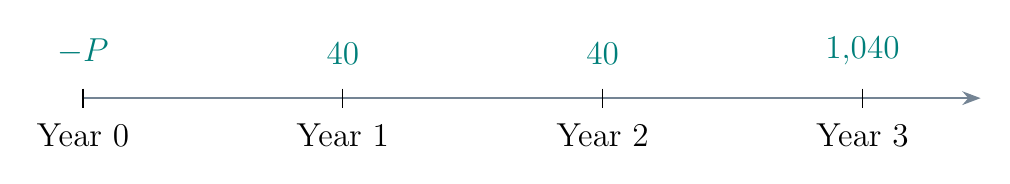
\begin{tikzpicture}[>=Stealth,every node/.style={font=\large,align=center}]\draw[->,Ink!60,thick](0,0)--(11.4,0);\foreach \x/\t/\pay in {0/0/{-P},3.3/1/40,6.6/2/40,9.9/3/{1{,}040}}{\draw(\x,.12)--(\x,-.12);\node[below]at(\x,-.2){Year \t};\node[above,Teal]at(\x,.3){$\pay$};}\end{tikzpicture}\end{center}\point{At maturity, the investor receives face value\par plus the final coupon.}
\end{frame}

% Slide 7: Face value and the price quote are different

\begin{frame}{Face value and the price quote are different}
\point{Teaching examples often use face value 100 or 1,000.}\[\text{Quote of 98 per 100 face}\quad\Rightarrow\quad980\text{ for }1{,}000\text{ face}.\]\eqnote{This example excludes accrued interest. Actual denominations depend on the instrument.}
\end{frame}

% Slide 8: A zero-coupon bond has one future payment

\begin{frame}{A zero-coupon bond has one future payment}
\point{$\spot{T}$: annual spot yield on a payment in T years.}\[\boxed{P=\frac{F}{(1+\spot{T})^T}.}\]\eqnote{A spot rate applies from today to the stated maturity.\par Annual compounding and certain repayment for this example.}
\end{frame}

% Slide 9: Discounting a face value of 1,000

\begin{frame}{Discounting a face value of 1,000}
\[F=1{,}000,\qquad T=2,\qquad\spot{2}=5\%.\]\[P=\frac{1{,}000}{1.05^2}=907.03.\]\point{Pay 907.03 now to receive 1,000 in two years.}
\end{frame}

% Slide 10: A coupon bond discounts every dated payment

\begin{frame}{A coupon bond discounts every dated payment}
\[P=\sum_{k=1}^{n}\frac{c_{\mathrm{coupon}}F}{(1+\bondyield)^k}+\frac{F}{(1+\bondyield)^n}.\]\begin{center}\begin{tabular}{@{}ll@{}}\toprule \textbf{Symbol} & \textbf{Meaning}\\\midrule $n$ & Number of annual coupon periods\\[2mm]
$k$ & Payment-year index\\[2mm]
$\bondyield$ & Single yield to maturity matching the bond price\\\bottomrule\end{tabular}\end{center}
\end{frame}

% Slide 11: The coupon-bond calculation

\begin{frame}{The coupon-bond calculation}
\[P=\frac{40}{1.05}+\frac{40}{1.05^2}+\frac{1{,}040}{1.05^3}=972.77.\]\point{A 4\% coupon with a 5\% yield gives a price below face value.}\eqnote{Annual payments, valued on a coupon date.}
\end{frame}

% Slide 12: Higher discount yields mean lower bond prices

\begin{frame}{Higher discount yields mean lower bond prices}
\begin{center}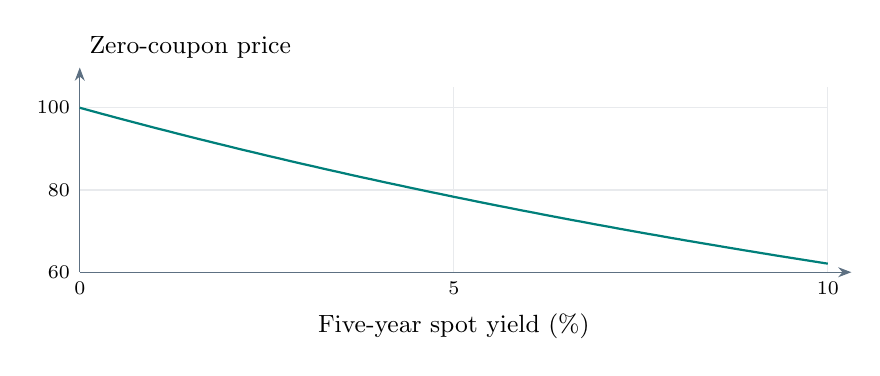
\begin{tikzpicture}[>=Stealth,every node/.style={font=\small}]
\draw[Ink!10] (0.000,0.000)--(0.000,2.350);\node[below,font=\scriptsize] at (0.000,0.000){0};
\draw[Ink!10] (4.750,0.000)--(4.750,2.350);\node[below,font=\scriptsize] at (4.750,0.000){5};
\draw[Ink!10] (9.500,0.000)--(9.500,2.350);\node[below,font=\scriptsize] at (9.500,0.000){10};
\draw[Ink!10] (0.000,0.000)--(9.500,0.000);\node[left,font=\scriptsize] at (0.000,0.000){60};
\draw[Ink!10] (0.000,1.044)--(9.500,1.044);\node[left,font=\scriptsize] at (0.000,1.044){80};
\draw[Ink!10] (0.000,2.089)--(9.500,2.089);\node[left,font=\scriptsize] at (0.000,2.089){100};
\draw[->,Ink!70] (0,0)--(9.8,0);\draw[->,Ink!70] (0,0)--(0,2.6);
\node[below] at (4.75,-.40){Five-year spot yield (\%)};\node[anchor=west] at (0,2.85){Zero-coupon price};
\draw[Teal,thick] plot coordinates {(0.000,2.089) (0.095,2.063) (0.190,2.037) (0.285,2.011) (0.380,1.986) (0.475,1.960) (0.570,1.935) (0.665,1.910) (0.760,1.885) (0.855,1.860) (0.950,1.835) (1.045,1.811) (1.140,1.787) (1.235,1.762) (1.330,1.738) (1.425,1.714) (1.520,1.690) (1.615,1.667) (1.710,1.643) (1.805,1.620) (1.900,1.597) (1.995,1.573) (2.090,1.550) (2.185,1.528) (2.280,1.505) (2.375,1.482) (2.470,1.460) (2.565,1.438) (2.660,1.415) (2.755,1.393) (2.850,1.371) (2.945,1.350) (3.040,1.328) (3.135,1.306) (3.230,1.285) (3.325,1.264) (3.420,1.242) (3.515,1.221) (3.610,1.200) (3.705,1.180) (3.800,1.159) (3.895,1.138) (3.990,1.118) (4.085,1.098) (4.180,1.077) (4.275,1.057) (4.370,1.037) (4.465,1.017) (4.560,0.998) (4.655,0.978) (4.750,0.958) (4.845,0.939) (4.940,0.920) (5.035,0.900) (5.130,0.881) (5.225,0.862) (5.320,0.843) (5.415,0.825) (5.510,0.806) (5.605,0.787) (5.700,0.769) (5.795,0.751) (5.890,0.732) (5.985,0.714) (6.080,0.696) (6.175,0.678) (6.270,0.660) (6.365,0.643) (6.460,0.625) (6.555,0.607) (6.650,0.590) (6.745,0.573) (6.840,0.555) (6.935,0.538) (7.030,0.521) (7.125,0.504) (7.220,0.487) (7.315,0.471) (7.410,0.454) (7.505,0.437) (7.600,0.421) (7.695,0.404) (7.790,0.388) (7.885,0.372) (7.980,0.356) (8.075,0.340) (8.170,0.324) (8.265,0.308) (8.360,0.292) (8.455,0.276) (8.550,0.261) (8.645,0.245) (8.740,0.230) (8.835,0.214) (8.930,0.199) (9.025,0.184) (9.120,0.169) (9.215,0.154) (9.310,0.139) (9.405,0.124) (9.500,0.109)};

\end{tikzpicture}\end{center}\eqnote{Hypothetical zero-coupon bond: face value 100, maturity five years, fixed cash flow.}
\end{frame}

% Slide 13: Duration measures local yield sensitivity

\begin{frame}{Duration measures local yield sensitivity}
\[\frac{\Delta P}{P}\approx-D_{\mathrm{mod}}\,\Delta\bondyield.\]\point{$D_{\mathrm{mod}}$: modified duration, the bond\textquotesingle s local price sensitivity.}\point{Duration 8 and a 0.50-point yield rise\par imply approximately $-8\times0.005=-4\%$.}
\end{frame}

% Slide 14: Treasury bills pay face value without periodic coupons

\begin{frame}{Treasury bills pay face value without periodic coupons}
\point{T-bills are short-term US Treasury securities,\par with original maturities of one year or less.}\[\text{Pay }98\text{ now}\quad\longrightarrow\quad\text{receive }100\text{ at maturity}.\]\[\text{Holding-period return}=\frac{100-98}{98}=2.04\%.\]
\end{frame}

% Slide 15: The yield curve is one date with many maturities

\begin{frame}{The yield curve is one date with many maturities}
\begin{center}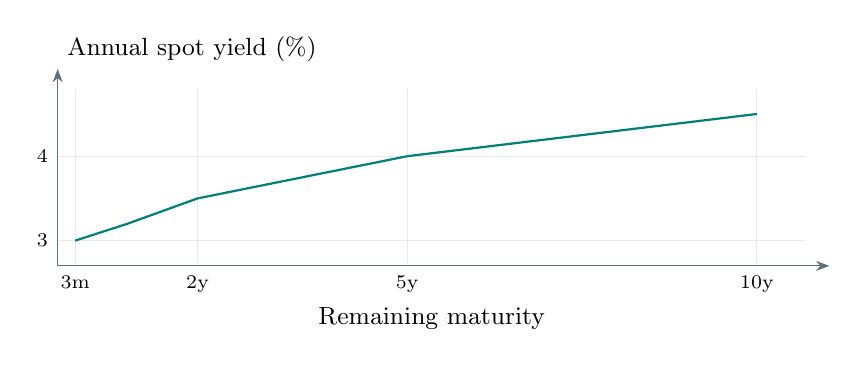
\begin{tikzpicture}[>=Stealth,every node/.style={font=\small}]
\draw[Ink!10] (0.222,0.000)--(0.222,2.250);\node[below,font=\scriptsize] at (0.222,0.000){3m};
\draw[Ink!10] (1.776,0.000)--(1.776,2.250);\node[below,font=\scriptsize] at (1.776,0.000){2y};
\draw[Ink!10] (4.439,0.000)--(4.439,2.250);\node[below,font=\scriptsize] at (4.439,0.000){5y};
\draw[Ink!10] (8.879,0.000)--(8.879,2.250);\node[below,font=\scriptsize] at (8.879,0.000){10y};
\draw[Ink!10] (0.000,0.321)--(9.500,0.321);\node[left,font=\scriptsize] at (0.000,0.321){3};
\draw[Ink!10] (0.000,1.393)--(9.500,1.393);\node[left,font=\scriptsize] at (0.000,1.393){4};
\draw[->,Ink!70] (0,0)--(9.8,0);\draw[->,Ink!70] (0,0)--(0,2.5);
\node[below] at (4.75,-.40){Remaining maturity};\node[anchor=west] at (0,2.75){Annual spot yield (\%)};
\draw[Teal,thick] plot coordinates {(0.222,0.321) (0.888,0.536) (1.776,0.857) (4.439,1.393) (8.879,1.929)};

\end{tikzpicture}\end{center}\eqnote{The horizontal axis is maturity. It is not the calendar path of policy rates.}
\end{frame}

% Slide 16: Yield curves can have different shapes

\begin{frame}{Yield curves can have different shapes}
\begin{center}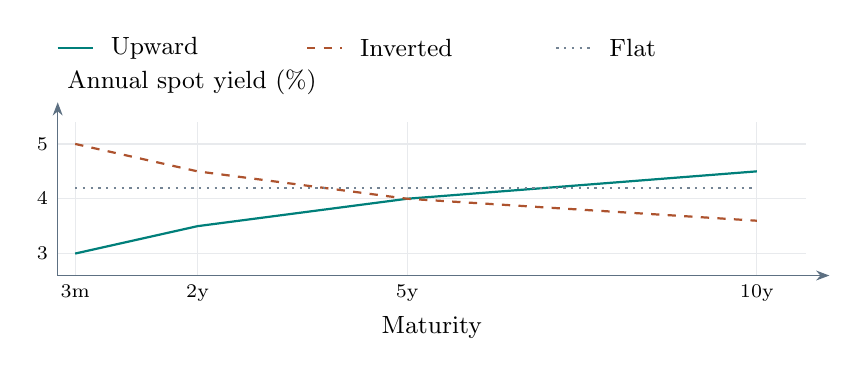
\begin{tikzpicture}[>=Stealth,every node/.style={font=\small}]
\draw[Ink!10] (0.222,0.000)--(0.222,1.950);\node[below,font=\scriptsize] at (0.222,0.000){3m};
\draw[Ink!10] (1.776,0.000)--(1.776,1.950);\node[below,font=\scriptsize] at (1.776,0.000){2y};
\draw[Ink!10] (4.439,0.000)--(4.439,1.950);\node[below,font=\scriptsize] at (4.439,0.000){5y};
\draw[Ink!10] (8.879,0.000)--(8.879,1.950);\node[below,font=\scriptsize] at (8.879,0.000){10y};
\draw[Ink!10] (0.000,0.279)--(9.500,0.279);\node[left,font=\scriptsize] at (0.000,0.279){3};
\draw[Ink!10] (0.000,0.975)--(9.500,0.975);\node[left,font=\scriptsize] at (0.000,0.975){4};
\draw[Ink!10] (0.000,1.671)--(9.500,1.671);\node[left,font=\scriptsize] at (0.000,1.671){5};
\draw[->,Ink!70] (0,0)--(9.8,0);\draw[->,Ink!70] (0,0)--(0,2.2);
\node[below] at (4.75,-.40){Maturity};\node[anchor=west] at (0,2.45){Annual spot yield (\%)};
\draw[Teal,thick] plot coordinates {(0.222,0.279) (1.776,0.627) (4.439,0.975) (8.879,1.323)};
\draw[Rust,thick,dashed] plot coordinates {(0.222,1.671) (1.776,1.323) (4.439,0.975) (8.879,0.696)};
\draw[Ink!60,dotted,thick] plot coordinates {(0.222,1.114) (8.879,1.114)};
\draw[Teal,thick] (0.0,2.89)--(0.45,2.89);\node[anchor=west,font=\small] at (0.55,2.89){Upward};
\draw[Rust,thick,dashed] (3.1666666666666665,2.89)--(3.6166666666666667,2.89);\node[anchor=west,font=\small] at (3.716666666666667,2.89){Inverted};
\draw[Ink!60,dotted,thick] (6.333333333333333,2.89)--(6.783333333333333,2.89);\node[anchor=west,font=\small] at (6.883333333333333,2.89){Flat};

\end{tikzpicture}\end{center}\eqnote{All shapes are hypothetical. A slope alone is not yet a forecast of future short rates.}
\end{frame}

% Slide 17: US and euro-area curve snapshot

\begin{frame}{US and euro-area curve snapshot}
\begin{center}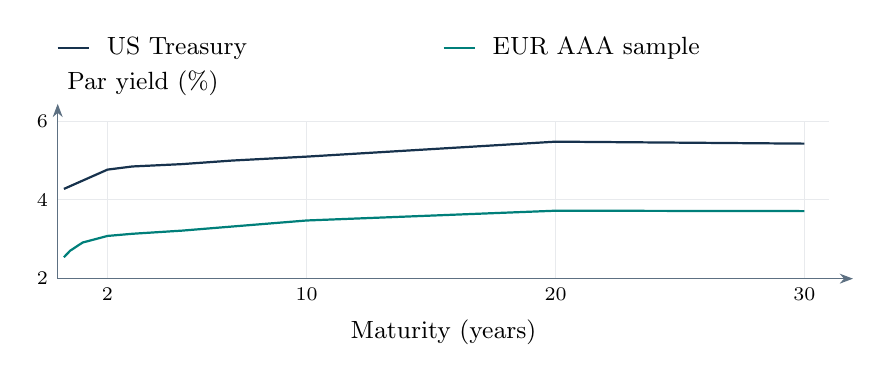
\begin{tikzpicture}[>=Stealth,every node/.style={font=\small}]
\draw[Ink!10] (0.6323,0.0000)--(0.6323,2.0000);\node[below,font=\scriptsize] at (0.6323,0.0000){2};
\draw[Ink!10] (3.1613,0.0000)--(3.1613,2.0000);\node[below,font=\scriptsize] at (3.1613,0.0000){10};
\draw[Ink!10] (6.3226,0.0000)--(6.3226,2.0000);\node[below,font=\scriptsize] at (6.3226,0.0000){20};
\draw[Ink!10] (9.4839,0.0000)--(9.4839,2.0000);\node[below,font=\scriptsize] at (9.4839,0.0000){30};
\draw[Ink!10] (0.0000,0.0000)--(9.8000,0.0000);\node[left,font=\scriptsize] at (0.0000,0.0000){2};
\draw[Ink!10] (0.0000,1.0000)--(9.8000,1.0000);\node[left,font=\scriptsize] at (0.0000,1.0000){4};
\draw[Ink!10] (0.0000,2.0000)--(9.8000,2.0000);\node[left,font=\scriptsize] at (0.0000,2.0000){6};
\draw[->,Ink!70] (0,0)--(10.100000000000001,0);\draw[->,Ink!70] (0,0)--(0,2.22);
\node[below] at (4.9,-.40){Maturity (years)};\node[anchor=west] at (0,2.48){Par yield (\%)};
\draw[Ink,thick] plot coordinates {(0.0790,1.1400) (0.1581,1.1750) (0.3161,1.2450) (0.6323,1.3850) (0.9484,1.4250) (1.5806,1.4550) (2.2129,1.5000) (3.1613,1.5500) (6.3226,1.7400) (9.4839,1.7150)};
\draw[Teal,thick] plot coordinates {(0.0790,0.2727) (0.1581,0.3550) (0.3161,0.4589) (0.6323,0.5427) (0.9484,0.5702) (1.5806,0.6103) (2.2129,0.6620) (3.1613,0.7390) (6.3226,0.8631) (9.4839,0.8580)};
\draw[Ink,thick] (0.0,2.93)--(0.4,2.93);\node[anchor=west,font=\small] at (0.5,2.93){US Treasury};
\draw[Teal,thick] (4.9,2.93)--(5.300000000000001,2.93);\node[anchor=west,font=\small] at (5.4,2.93){EUR AAA sample};
\end{tikzpicture}\end{center}\eqnote{US: 15 October 2026. EUR: latest verified 14 October. Different currencies and issuer samples.}
\end{frame}

% Slide 18: Spot, forward and coupon-bond yields

\begin{frame}{Spot, forward and coupon-bond yields}
\begin{center}\begin{tabular}{@{}p{.33\textwidth}p{.59\textwidth}@{}}\toprule \textbf{Rate} & \textbf{What is fixed today?}\\\midrule $\spot{T}$ & Price of a zero-coupon payment at T\\[2mm]
$\forward{T_1}{T_2}$ & Rate for a future lending interval\\[2mm]
$\bondyield$ & One yield matching a coupon bond\textquotesingle s price\\\bottomrule\end{tabular}\end{center}\eqnote{T, T1 and T2 are future dates measured in years from today.}
\end{frame}

% Slide 19: Two ways to lock a two-year payoff

\begin{frame}{Two ways to lock a two-year payoff}
\point{Route A: buy a two-year zero-coupon bond.}\point{Route B: invest for one year, then reinvest\par at a second-year rate locked today.}\eqnote{Same initial investment, currency, credit and final payment date.}
\end{frame}

% Slide 20: No-arbitrage makes the locked payoffs match

\begin{frame}{No-arbitrage makes the locked payoffs match}
\[\boxed{(1+\spot{2})^2=(1+\spot{1})(1+\forward{1}{2}).}\]\point{If locked returns differed, borrow along the cheaper route\par and lend along the more profitable route.}
\end{frame}

% Slide 21: Calculating the implied forward

\begin{frame}{Calculating the implied forward}
\[\spot{1}=4\%,\qquad\spot{2}=5\%.\]\[\forward{1}{2}=\frac{1.05^2}{1.04}-1=6.01\%.\]\point{Both locked routes turn 100 today into 110.25 in two years.}
\end{frame}

% Slide 22: A locked forward is not a guaranteed forecast

\begin{frame}{A locked forward is not a guaranteed forecast}
\point{The forward rate is a contract price today.}\point{Next year\textquotesingle s realised short rate remains uncertain.}\eqnote{Risk premia can separate an implied forward from the physical expected future rate.}
\end{frame}

% Slide 23: A long yield contains a path and a premium

\begin{frame}{A long yield contains a path and a premium}
\point{Expected average short rate over the bond\textquotesingle s life.}\point{Plus a term premium for holding long-duration exposure.}\[3.0\%+0.5\%=3.5\%\quad\text{in a hypothetical example}.\]
\end{frame}

% Slide 24: Writing the yield decomposition mathematically

\begin{frame}{Writing the yield decomposition mathematically}
\[\spot{n}\approx\frac1n\sum_{k=0}^{n-1}\mathbb E_t R_{t+k}^{\mathrm{policy}}+TP(n).\]\begin{center}\begin{tabular}{@{}ll@{}}\toprule \textbf{Symbol} & \textbf{Meaning}\\\midrule $n$ & Maturity in years\\[2mm]
$\mathbb E_t$ & Expectation formed today\\[2mm]
$TP(n)$ & Term premium for that maturity\\\bottomrule\end{tabular}\end{center}
\end{frame}

% Slide 25: Today's rate and a ten-year yield can move differently

\begin{frame}{Today's rate and a ten-year yield can move differently}
\point{A cut today changes only part of the expected future path.}\point{Later expected rates or the term premium can rise\par enough to raise the long yield.}\eqnote{A policy decision does not fix the entire yield curve.}
\end{frame}

% Slide 26: Exercise: a cut today with a bond sell-off

\begin{frame}{Exercise: a cut today with a bond sell-off}
\point{Expected average short rates over ten years rise 0.10 points.}\point{The ten-year term premium rises 0.20 points.}\point{Predict the yield move and the duration-8 price change.}
\end{frame}

% Slide 27: The decomposition gives the answer

\begin{frame}{The decomposition gives the answer}
\[\Delta\spot{10}\approx0.10+0.20=0.30\text{ percentage points}.\]\[\frac{\Delta P}{P}\approx-8\times0.003=-2.4\%.\]\point{The long yield rises and the bond loses value\par in this specified scenario.}
\end{frame}

% Slide 28: A curve-slope exercise
\section[A curve-slope exercise]{A curve-slope exercise}
\begin{frame}[plain]
{\color{Gold}\large LECTURE 3}\par\vspace{9mm}{\Huge\bfseries A curve-slope exercise}\par\vspace{7mm}{\Large How can two bond positions express a relative rate view?}
\end{frame}

% Slide 29: A curve view needs two maturity forecasts

\begin{frame}{A curve view needs two maturity forecasts}
\begin{center}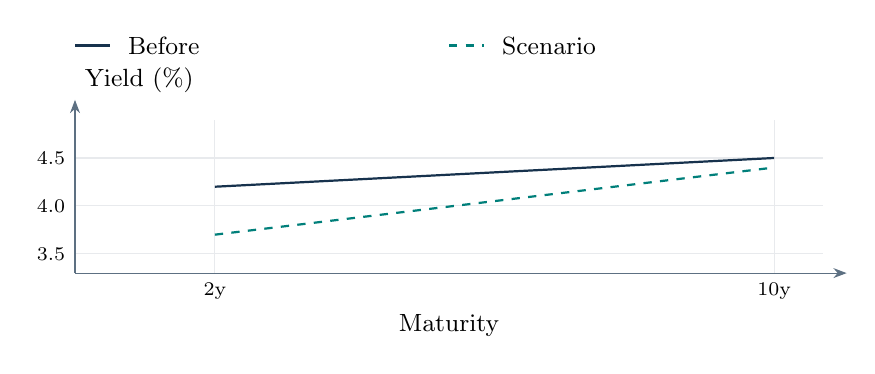
\begin{tikzpicture}[>=Stealth,every node/.style={font=\small}]
\draw[Ink!10] (1.776,0.000)--(1.776,1.950);\node[below,font=\scriptsize] at (1.776,0.000){2y};
\draw[Ink!10] (8.879,0.000)--(8.879,1.950);\node[below,font=\scriptsize] at (8.879,0.000){10y};
\draw[Ink!10] (0.000,0.244)--(9.500,0.244);\node[left,font=\scriptsize] at (0.000,0.244){3.5};
\draw[Ink!10] (0.000,0.853)--(9.500,0.853);\node[left,font=\scriptsize] at (0.000,0.853){4.0};
\draw[Ink!10] (0.000,1.462)--(9.500,1.462);\node[left,font=\scriptsize] at (0.000,1.462){4.5};
\draw[->,Ink!70] (0,0)--(9.8,0);\draw[->,Ink!70] (0,0)--(0,2.2);
\node[below] at (4.75,-.40){Maturity};\node[anchor=west] at (0,2.45){Yield (\%)};
\draw[Ink,thick] plot coordinates {(1.776,1.097) (8.879,1.462)};
\draw[Teal,thick,dashed] plot coordinates {(1.776,0.488) (8.879,1.341)};
\draw[Ink,thick] (0.0,2.89)--(0.45,2.89);\node[anchor=west,font=\small] at (0.55,2.89){Before};
\draw[Teal,thick,dashed] (4.75,2.89)--(5.2,2.89);\node[anchor=west,font=\small] at (5.3,2.89){Scenario};

\end{tikzpicture}\end{center}\eqnote{Both yields fall. The two-year yield falls more. Hypothetical matched bond-yield moves.}
\end{frame}

% Slide 30: This is a bull steepening

\begin{frame}{This is a bull steepening}
\[\text{Slope}=\text{ten-year yield}-\text{two-year yield}.\]\[0.30\text{ points}\quad\longrightarrow\quad0.70\text{ points}.\]\point{Bull: yields fall and bond prices rise.\par Steepening: the long-minus-short yield spread increases.}
\end{frame}

% Slide 31: Expressing the relative view with bonds

\begin{frame}{Expressing the relative view with bonds}
\point{Buy the two-year bond: benefit if its yield falls.}\point{Short the ten-year bond: lose if its yield falls.}\point{Size the legs so the stronger two-year rally\par can outweigh the ten-year loss.}
\end{frame}

% Slide 32: DV01 puts the two legs on comparable terms

\begin{frame}{DV01 puts the two legs on comparable terms}
\point{One basis point (bp) is 0.01 percentage point, or 0.0001.}\[DV01\approx V D_{\mathrm{mod}}\times0.0001.\]\point{$V$: current market value.\par DV01: approximate currency price change for a one-bp yield move.}
\end{frame}

% Slide 33: Exercise: choose the size of the short leg

\begin{frame}{Exercise: choose the size of the short leg}
\begin{center}\begin{tabular}{@{}llll@{}}\toprule \textbf{Position} & \textbf{Market value} & \textbf{Duration} & \textbf{DV01}\\\midrule Long two-year & 1,000,000 & 1.8 & 180 / bp\\[2mm]
Short ten-year & ? & 8.0 & 180 / bp\\\bottomrule\end{tabular}\end{center}\point{What ten-year market value matches the long leg\textquotesingle s DV01?}
\end{frame}

% Slide 34: Equal DV01 requires unequal market values

\begin{frame}{Equal DV01 requires unequal market values}
\[V_{\mathrm{short}}=\frac{180}{8\times0.0001}=225{,}000.\]\begin{center}\begin{tabular}{@{}lll@{}}\toprule \textbf{Position} & \textbf{Market value} & \textbf{Signed DV01}\\\midrule Long two-year & 1,000,000 & +180 / bp\\[2mm]
Short ten-year & 225,000 & -180 / bp\\\bottomrule\end{tabular}\end{center}\eqnote{Approximately neutral to a small parallel yield move at inception.}
\end{frame}

% Slide 35: Work out the scenario profit and loss

\begin{frame}{Work out the scenario profit and loss}
\begin{center}\begin{tabular}{@{}lll@{}}\toprule \textbf{Leg} & \textbf{Yield move} & \textbf{Approximate P\&L}\\\midrule Long two-year & -50 bp & $+180\times50=+9{,}000$\\[2mm]
Short ten-year & -10 bp & $-180\times10=-1{,}800$\\[2mm]
Combined & 40 bp steepening & $+7{,}200$\\\bottomrule\end{tabular}\end{center}\eqnote{Local duration calculation, before carry, financing, costs and convexity.}
\end{frame}

% Slide 36: Counterfactual: what would make this trade lose?

\begin{frame}{Counterfactual: what would make this trade lose?}
\point{The ten-year minus two-year yield spread narrows instead.}\point{An expected cut is already priced, so the curve does not move as hoped.}\point{Financing, carry and imperfect hedging can overwhelm the gain.}
\end{frame}

% Slide 37: Further reading
\section[Reading]{Reading}
\begin{frame}{Further reading}
\point{Dmitriy Sergeyev, Bocconi 30054 course materials.}\point{Krugman, Obstfeld \& Melitz, \emph{International Economics}.}\point{Source links and worked answers accompany each slide in the notes.}
\end{frame}
\end{document}
